\subsection{Sprachkonzepte}
    Dieses Kapitel beschreibt, wie sich die Konzepte der Domäne
    (siehe z. B. Kapitel \ref{section:conceptClassesFeaturesSelectors})
    in Sprachkonzepten wiederspiegeln.
    Auch hier erfolgt die Beschreibung getrennt für die Konzepte Klassen,
    Features und Selektoren.

    Für diese Konzepte bietet die Sprache Linguistic Abstractions
    \cite[Kapitel 4.1, 4.1.2]{voelter:DslEngineering}.
    % TODO: Erklären!

    Abbildung \ref{image:dslClasses} zeigt das Modell der Konzepte für Klassen.

    \begin{figure}[htb]
        \centering
        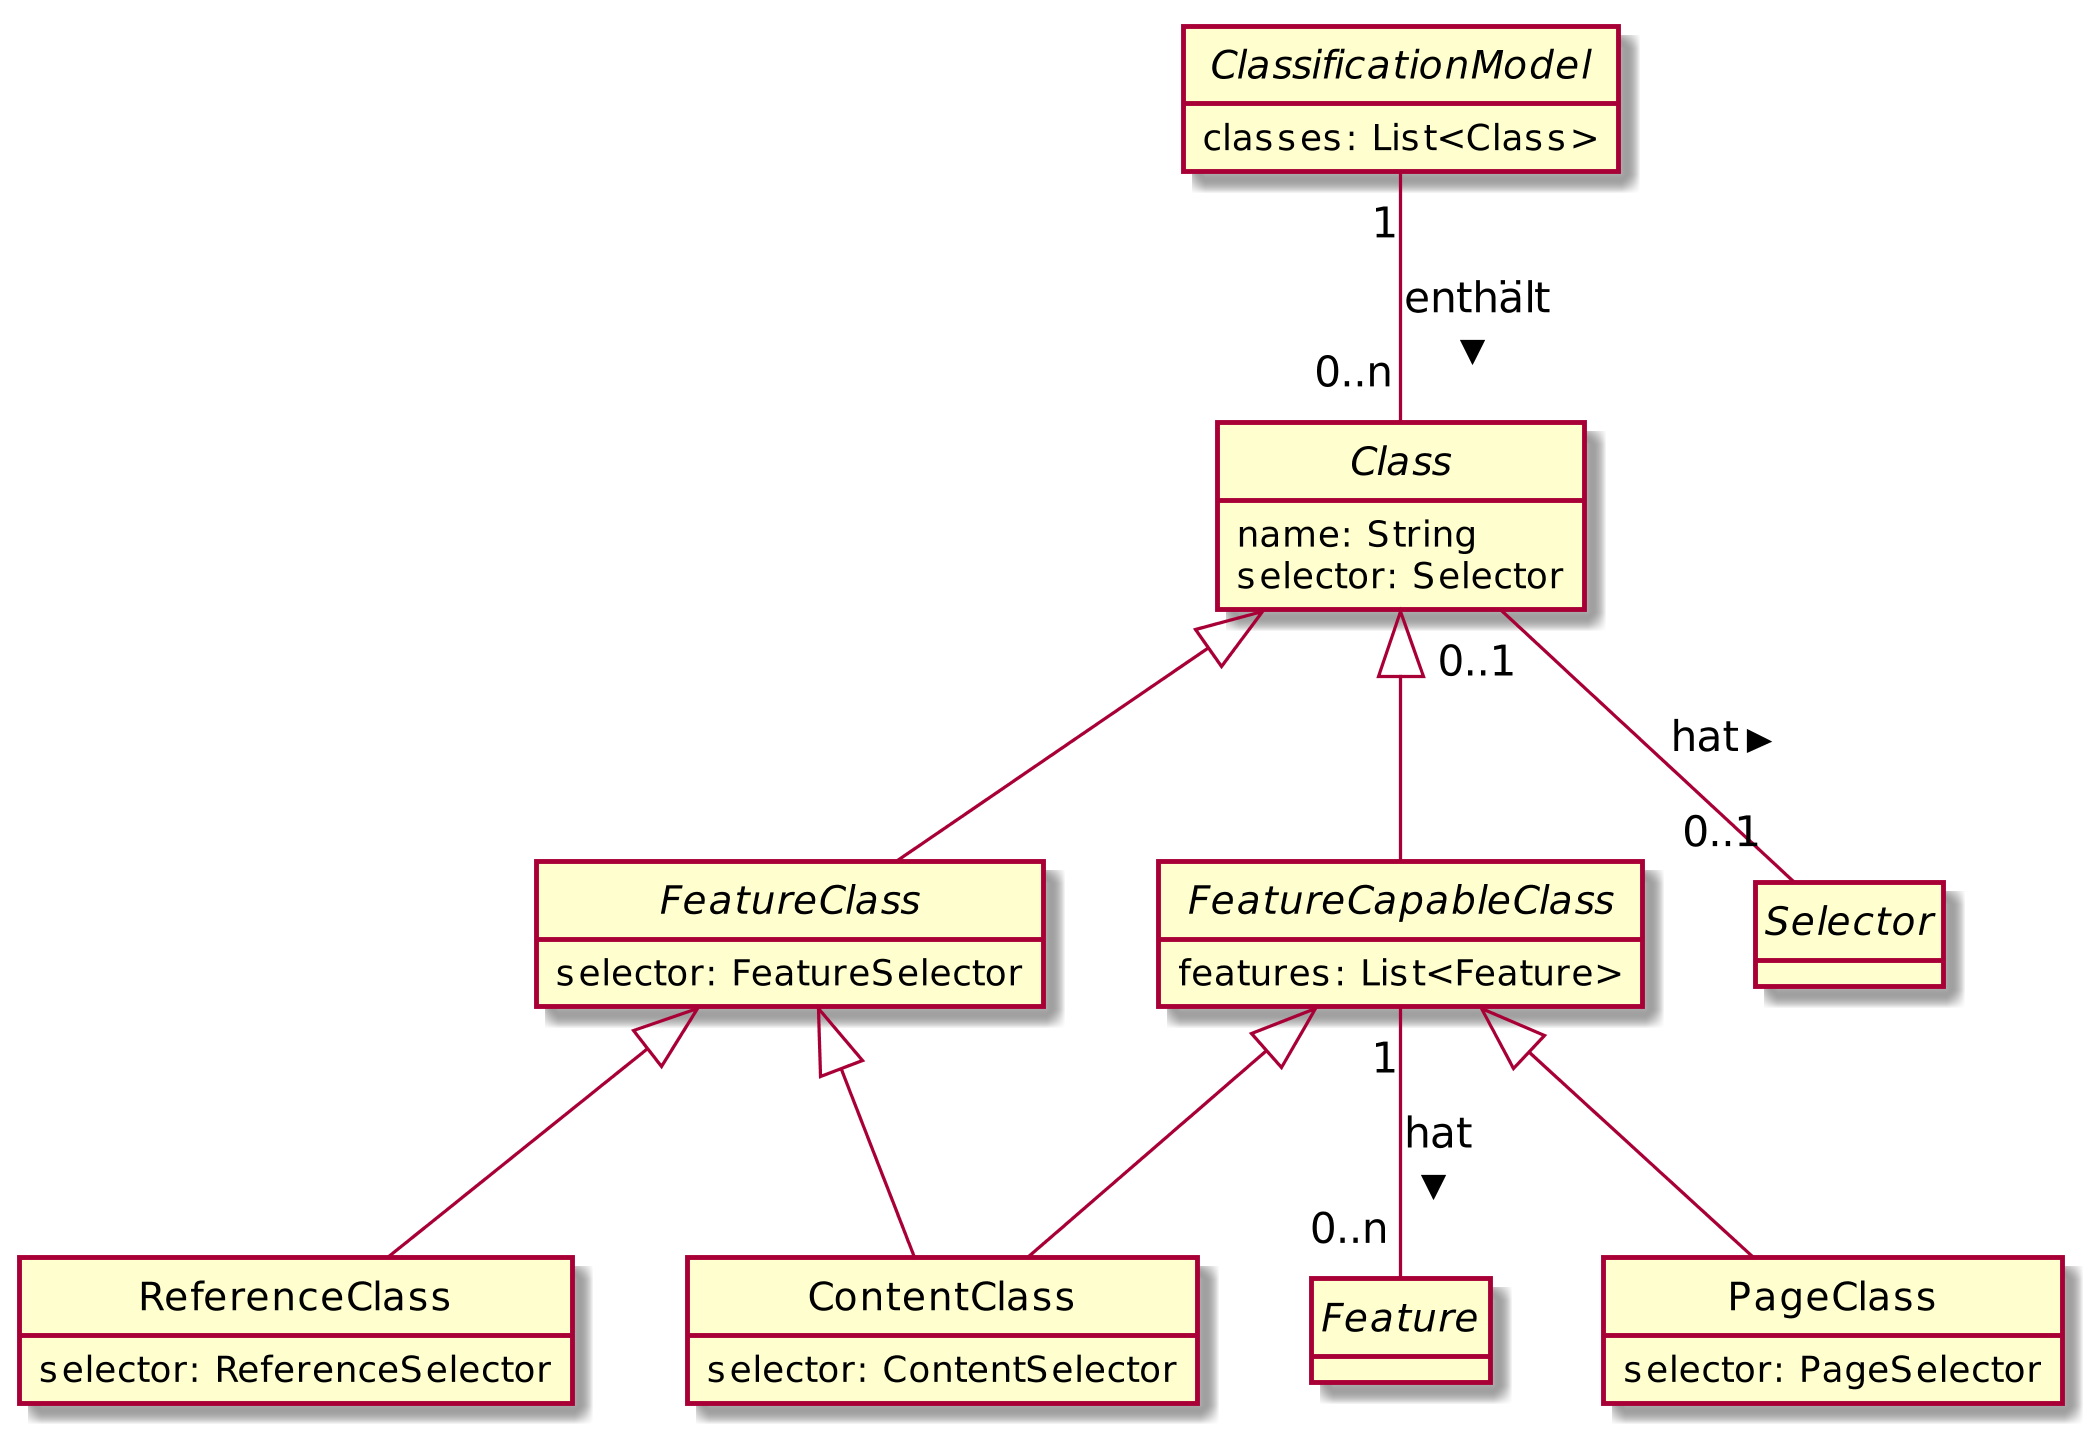
\includegraphics[width=\textwidth]{../resources/dsl/classes.png}
        \caption{Klassen in der DSL}
        \label{image:dslClasses}
    \end{figure}

    Klassen werden durch das abstrakte Konzept "`Class"' dargestellt,
    von denen es gemäß der Domänenkonzepte drei konkrete Ausprägungen in der Sprache
    existieren: "`PageClass"', "`ContentClass"' und "`ReferenceClass"'.
    Sämtliche Klassendefinitionen sind in Konzept "`ClassificationModel"' enthalten.

    Jede Klasse besitzt einen Namen und einen Selektor,
    der ausgenommen von PageClass optional ist.
    Selektoren werden durch das Konzept "`Selector"' repräsentiert.
    Für Content- und ReferenceClass stellt ein Selektor einen Standardwert
    für Features mit dieser Klasse dar.
    Da nicht jeder Selektor für jede Klasse geeignet ist,
    erwarten die einzelnen Klassentypen verschiedene Selektortypen:
    "`PageSelector"', "`ContentSelector"' und "`ReferenceSelector"'.
    Auf Selektoren wird weiter unten eingegangen.

    Seiten- und Inhaltsklassen können Features besitzen.
    Für diese Eigenschaft führt die Sprache das Konzept "`FeatureCapableClass"' ein,
    welches eine Ableitung von "`Class"' darstellt.
    Page- und ContentClass erben deshalb nicht direkt von "`Class"',
    sondern sondern indirekt über "`FeatureCapableClass"'.

    Gleichzeitig sind nur Inhalts- und Referenzklassen geeignet als Klassen
    von Features. Für diese Eigenschaft enthält die Sprache das Konzept "`FeatureClass"',
    welches ebenfalls von "`Class"' erbt und das Oberkonzept von Content- und ReferenceClass ist.

    Features werden in der Sprache durch das gleichnamige abstrakte Konzept repräsentiert,
    was Abbildung \ref{image:dslFeatures} veranschaulicht.

    \begin{figure}[htb]
        \centering
        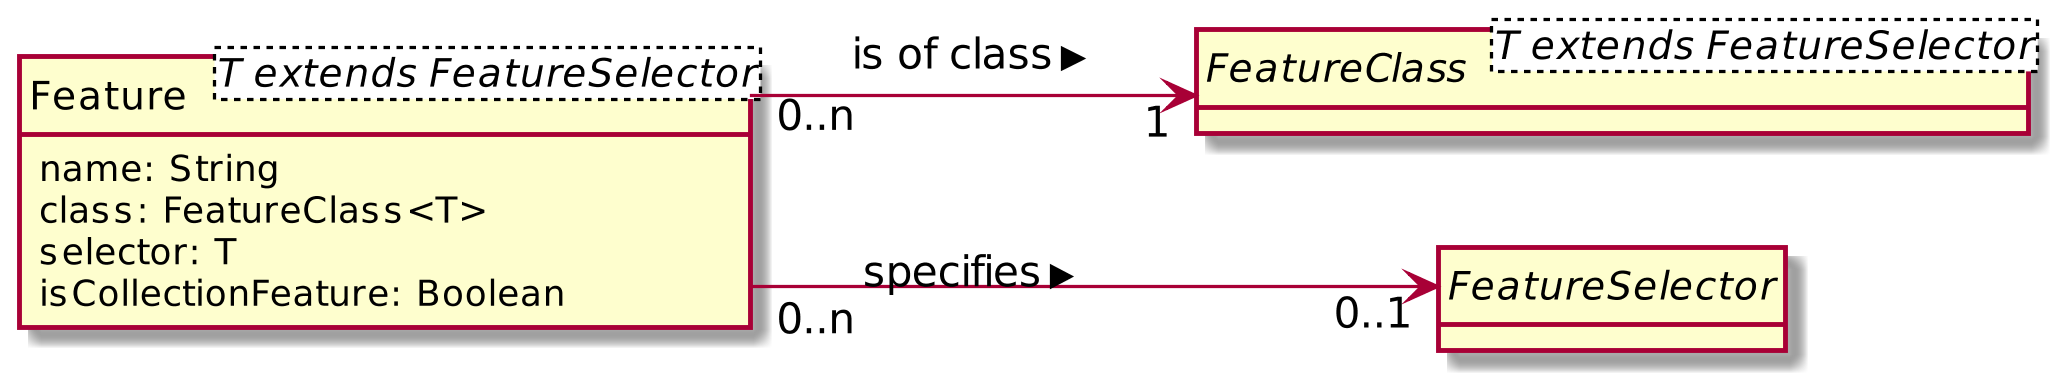
\includegraphics[width=\textwidth]{../resources/dsl/features.png}
        \caption{Features in der DSL}
        \label{image:dslFeatures}
    \end{figure}

    Analog zum Domänenkonzept besitzt jedes Feature in der Sprache einen Namen
    und eine Klasse, welche vom oben vorgestellten Typ "`FeatureClass"' sein muss.
    An dieser Stelle ist also eine Cross-Reference. Die einzige, die notwendig ist.
    Des Weiteren kann ein Feature einen Selektor besitzen, der den Selektor der
    Klasse überschreibt (siehe Konzeptkapitel, oder?).
    Da nicht jeder Selektor ist für jedes Feature geeignet ist (hängt von FeatureClass ab),
    führt die Sprache hierfür das Konzept "`FeatureSelector"' ein (sieh unten).
    Die Sprache besitzt zwei konkrete Ableitung von "`Feature"':
    "`ScalarFeature"' und "`CollectionFeature"', die die entsprechend ein- bzw. mehrelementige Features darstellen.
    Aus Sicht der Sprache ist das lediglich ein Flag, weshalb keine großartige Unterscheidung notwendig ist.
    Eine Unterscheidung zwischen Content- und ReferenceFeatures ist nicht notwendig,
    da das klar durch die konkrete FeatureClass festgelegt ist.

    Zuletzt bietet die Sprache Konzepte zur Definition von Selektoren,
    die vereinzelt schon angesprochen wurden.
    Eine vollständige Übersicht bietet Abbildung \ref{image:dslSelectors}.

    \begin{figure}[htb]
        \centering
        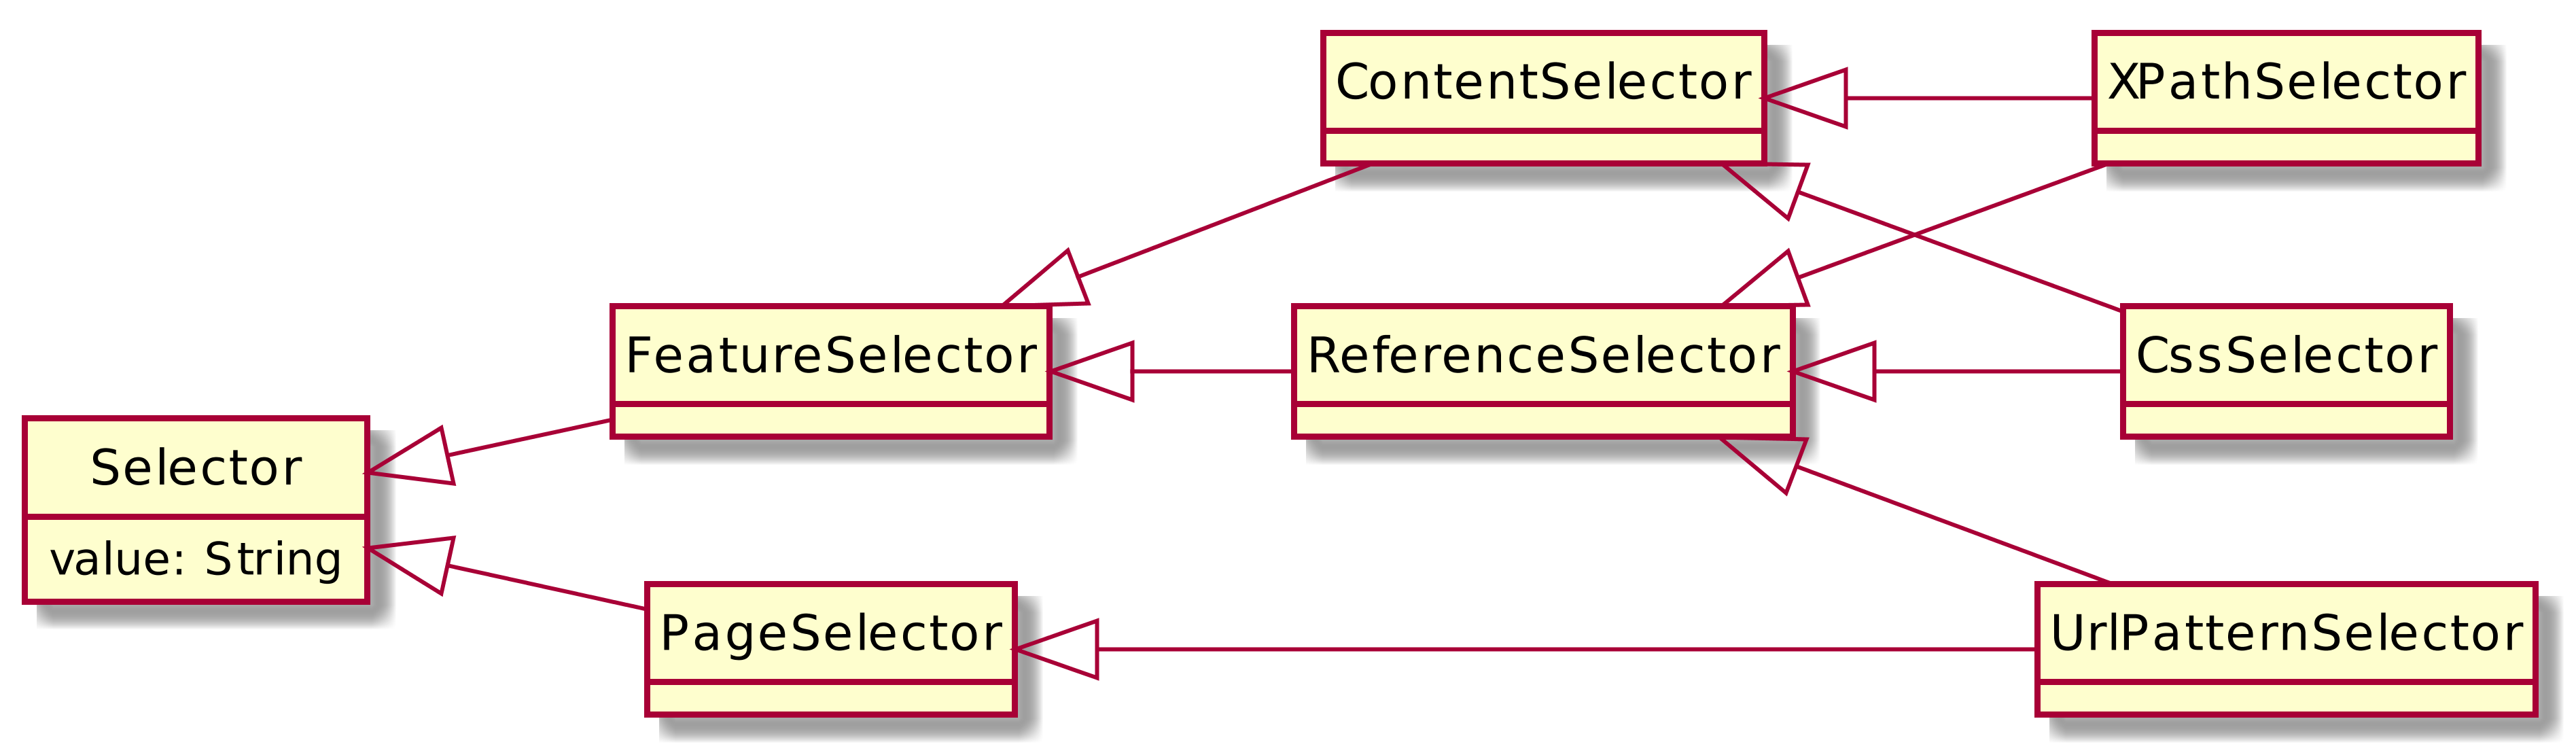
\includegraphics[width=\textwidth]{../resources/dsl/selectors.png}
        \caption{Selektoren in der DSL}
        \label{image:dslSelectors}
    \end{figure}

    Das abstrakte Konzept "`Selector"' entspricht dem gleichnamigen Domänenkonzept.
    Die Sprache enthält abstrakte Ableitungen von diesem Konzept,
    mit denen Selektoren nach ihrer Eignung für die verschiedenen Klassentypen
    getrennt werden. Deshalb gibt es "`PageSelector"', "`ContentSelector"' und "`ReferenceSelector"'.
    Die vom Klassifizierungssystem unterstützten Selektoren wurden schon in Kapitel
    \ref{section:conceptSupportedSelectors} beschrieben.
    Dementsprechend bietet die Sprache drei konkrete Selektoren:
    "`CssSelector"', "`XPathSelector"' und "`UrlPatternSelector"'.

    Wie oben beschrieben ist ein weiterer relevanter Aspekt, welche Selektoren
    für Features geeignet sind.
    Da Features nur Inhalts- oder Referenzklassen sein können,
    sind entsprechend nur ContentSelector und ReferenceSelector für Features geeignet.
    Deshalb stellen diese Konzepte Ableitungen vom abstrakten Konzept "`FeatureSelector"' dar,
    welches wie oben erwähnt in Feature genutzt wird.